% =============================================================================
\section{The Player and Interaction}\label{sec:interaction}
The user controls a person (the man model of \Cref{sec:humans}) who walks through the scene and operates the
machines by looking at a part and pressing \textbf{E} or the left mouse button. This section explains how the
player moves, how the program finds the part that is looked at, and how every object reacts.

\subsection{Movement of the player}\label{sec:camera}
\paragraph{Walking.} The player has a position $\mathbf{p}$ (the feet), a yaw angle $\psi$ (turning left and right)
and a pitch angle $\theta$ (looking up and down). Moving the mouse by $(\Delta m_x,\Delta m_y)$ pixels changes
\[
\psi \leftarrow \psi - 0.12\,\Delta m_x,\qquad \theta \leftarrow \mathrm{clamp}(\theta - 0.12\,\Delta m_y,\ -85^\circ,\ 85^\circ).
\]
The keys W, S, A, D give a forward input $w\in\{-1,0,1\}$ and a sideways input $a\in\{-1,0,1\}$. The forward and the
right direction on the ground follow the yaw:
\[
\mathbf{f} = (\sin\psi,\ 0,\ \cos\psi),\qquad \mathbf{r} = (-\cos\psi,\ 0,\ \sin\psi),\qquad
\mathbf{p} \leftarrow \mathbf{p} + \operatorname{normalize}(w\,\mathbf{f} + a\,\mathbf{r})\; v\,\Delta t,
\]
with the speed $v=2.4$ m/s (walking) or $5.0$ m/s (Shift, running). Gravity and jumping act on the height:
$v_y \leftarrow v_y - 12\,\Delta t$, $p_y \leftarrow p_y + v_y\Delta t$, and $p_y$ never goes below the terrain height; Space
sets $v_y=4.6$ m/s. While walking, the walk phase grows by $7\,\Delta t$ and drives the body animation of
\Cref{sec:humans} and a small head bob $0.028\sin(2\varphi)$ of the first-person camera.

\paragraph{Collision.} The player is a circle of radius $r=0.3$ m on the ground. Walls, machines, furniture and cars are
oriented boxes with a height range; tree trunks, posts and people are circles. To push the player out of a box, the
centre is moved into the box's own frame (rotation by $-yaw_{box}$), the nearest point of the box is found by clamping,
\[
\mathbf{q}=\mathrm{clamp}(\mathbf{p}_{local},\,-\mathbf{h},\,\mathbf{h}),\qquad
\text{if } |\mathbf{p}_{local}-\mathbf{q}|<r:\quad \mathbf{p}_{local} \leftarrow \mathbf{q} + r\,\frac{\mathbf{p}_{local}-\mathbf{q}}{|\mathbf{p}_{local}-\mathbf{q}|},
\]
and the result is turned back. Two circles are separated in the same way along the line between their centres.
The test is repeated three times per frame so corners work, and a box only counts when it overlaps the player's
height, so the player can walk under a table top. The sliding doors switch their box off while they are open.

\paragraph{Cameras.} Key V cycles through three cameras (\Cref{fig:cameras}):
\begin{itemize}
  \item \textbf{First person}: the camera is at eye height and looks along the view direction:
        \[\mathbf{e}=\mathbf{p}+(0,\,1.62,\,0),\qquad \mathbf{d}=(\sin\psi\cos\theta,\ \sin\theta,\ \cos\psi\cos\theta).\]
  \item \textbf{Third person}: the body is visible; the camera is placed $3.4$ m behind the head along $-\mathbf{d}$ and
        $0.35$ m higher. A ray from the head to the camera is tested against the collision boxes and the camera moves
        closer when a wall is in the way.
  \item \textbf{Free camera}: flies without collision (W A S D, Space, Ctrl) to inspect the scene, for example with
        the roof cut-away view.
\end{itemize}
The mouse wheel changes the field of view $f$ between $25^\circ$ and $110^\circ$, which changes the $1/\tan(f/2)$ terms of
the projection matrix (\Cref{sec:transform}).
\begin{figure}[H]
\centering
\begin{subfigure}{0.49\linewidth}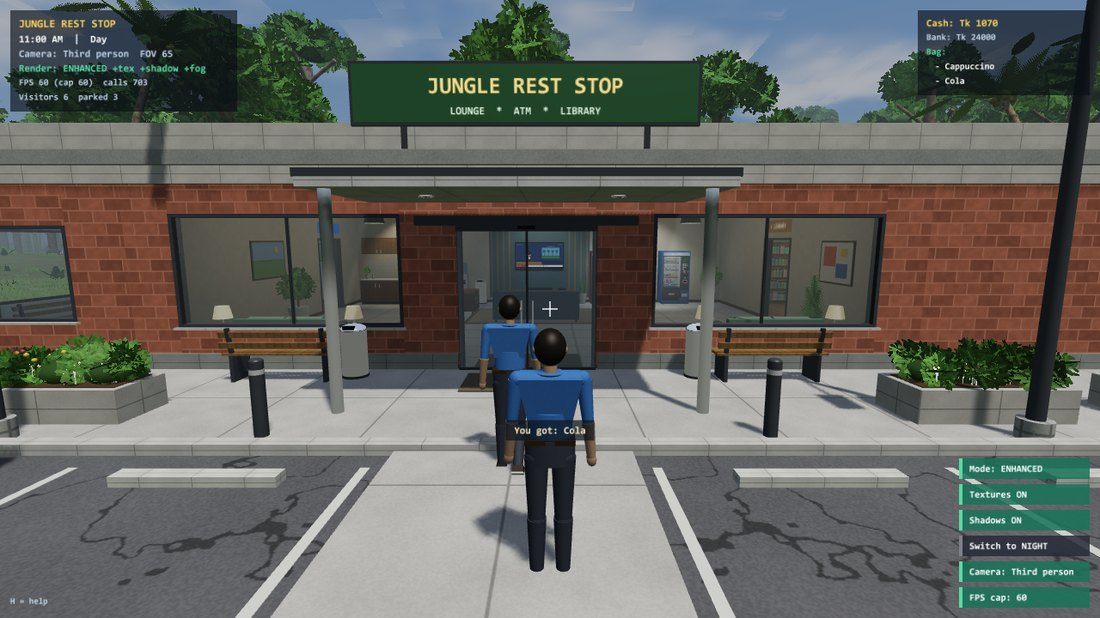
\includegraphics[width=\linewidth]{play_walk_1}\caption{Third person: walking to the entrance}\end{subfigure}
\begin{subfigure}{0.49\linewidth}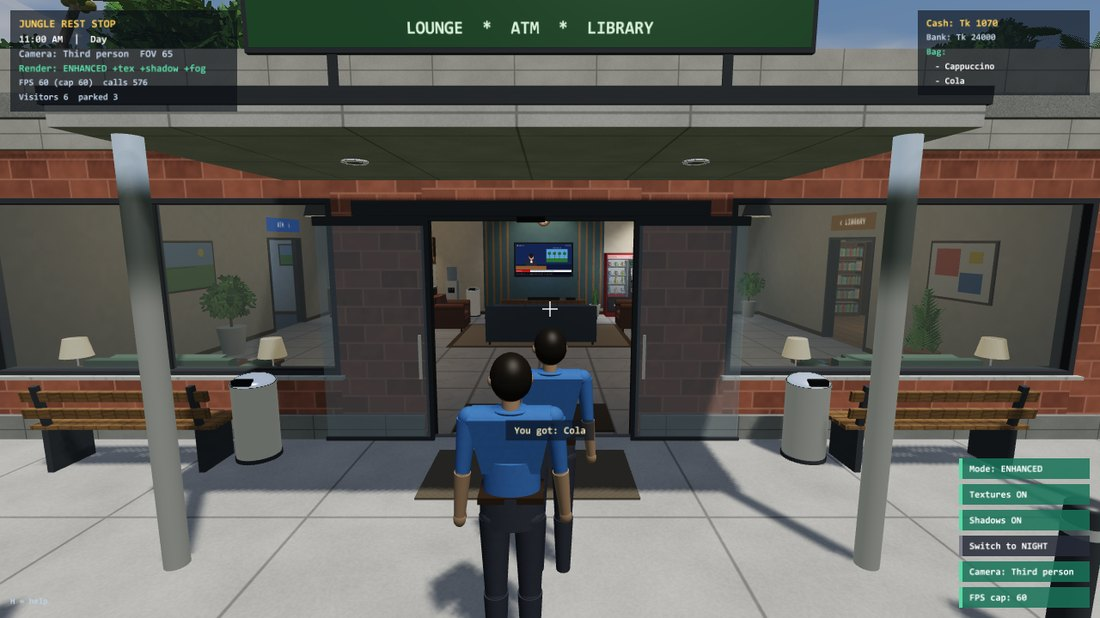
\includegraphics[width=\linewidth]{play_door}\caption{The sliding doors open in front of the player}\end{subfigure}
\begin{subfigure}{0.49\linewidth}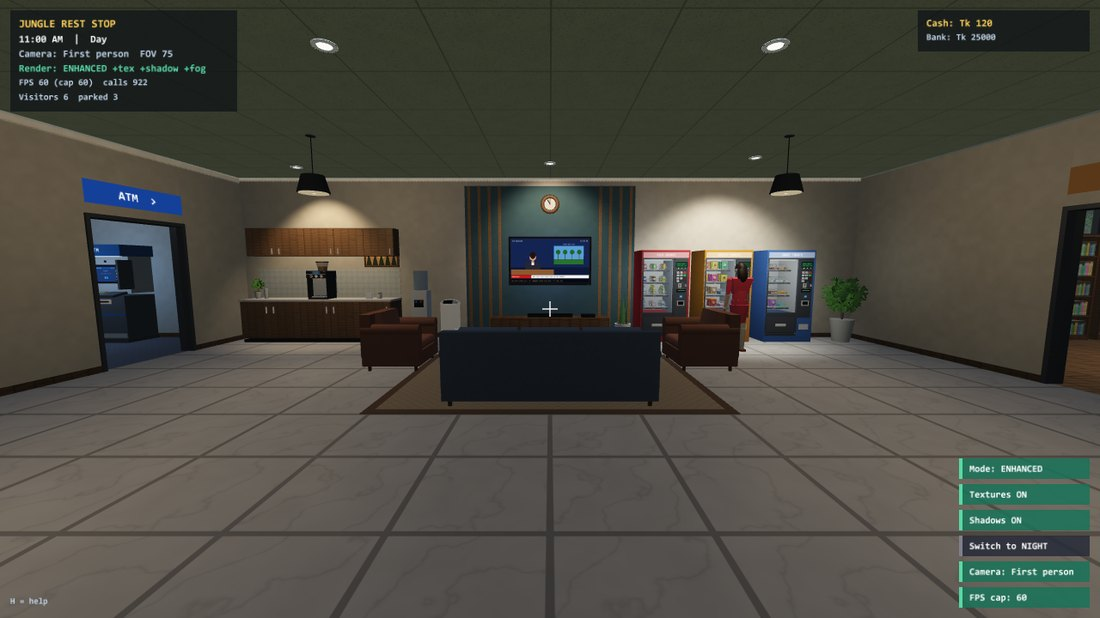
\includegraphics[width=\linewidth]{lounge_day}\caption{First person}\end{subfigure}
\begin{subfigure}{0.49\linewidth}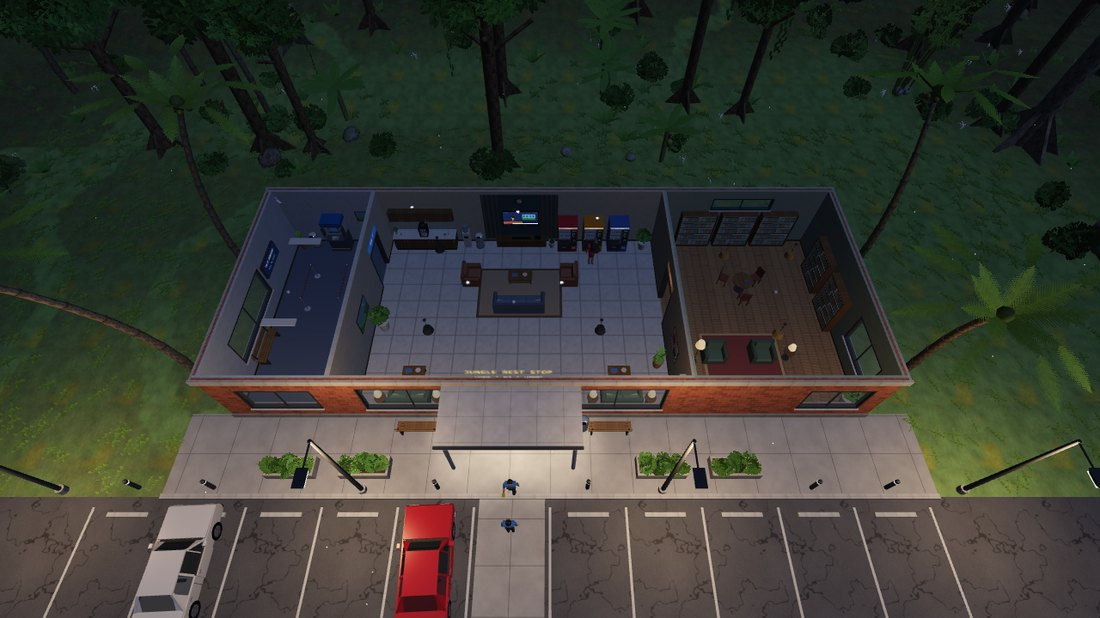
\includegraphics[width=\linewidth]{cutaway_night}\caption{Free camera, roof cut-away, night}\end{subfigure}
\begin{subfigure}{0.32\linewidth}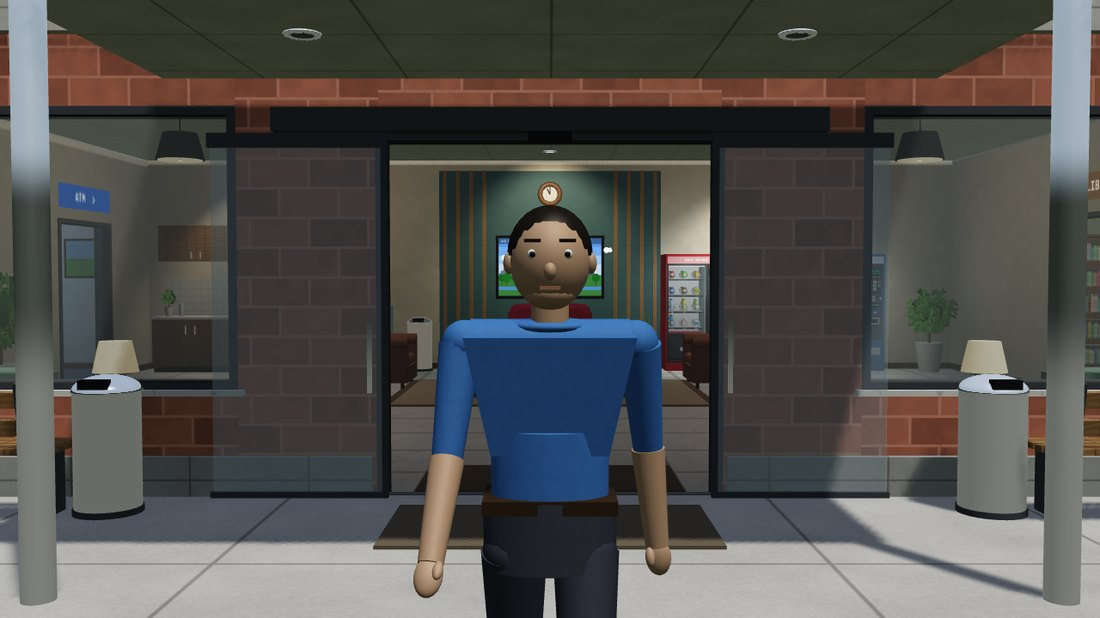
\includegraphics[width=\linewidth]{fov_35}\caption{FOV 35$^\circ$}\end{subfigure}
\begin{subfigure}{0.32\linewidth}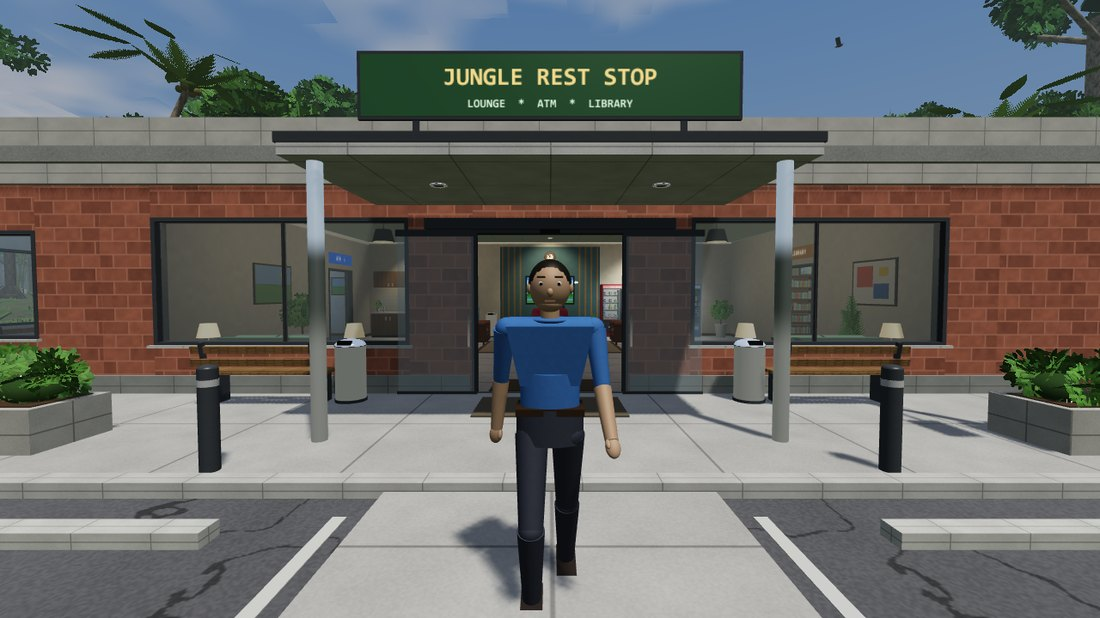
\includegraphics[width=\linewidth]{fov_70}\caption{FOV 70$^\circ$}\end{subfigure}
\begin{subfigure}{0.32\linewidth}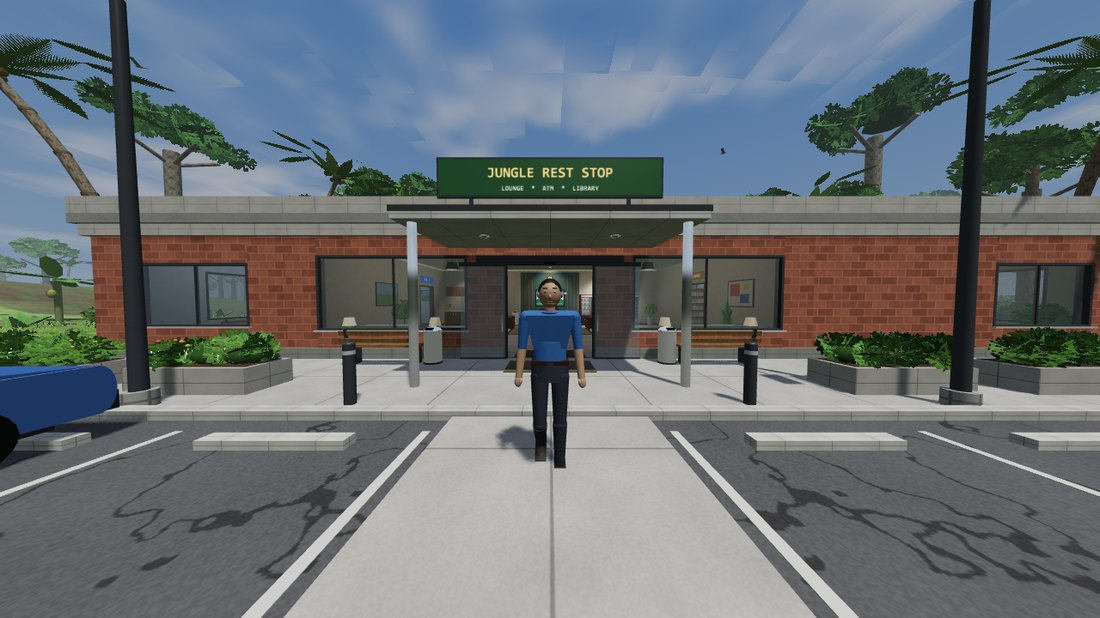
\includegraphics[width=\linewidth]{fov_100}\caption{FOV 100$^\circ$}\end{subfigure}
\caption{Camera modes and field of view.}\label{fig:cameras}
\end{figure}

\subsection{Object picking}
Every interactive part (buttons, slots, the flap, switches, the TV, the aquarium) registers an \emph{oriented box}
every frame: its matrix $M$ and its half size $\mathbf{h}$. A ray starts at the camera, $\mathbf{o}=\mathbf{e}$, and goes
through the centre of the screen in the view direction $\mathbf{d}$. For each box the ray is moved into the box's own
frame, $\mathbf{o}'=M^{-1}\mathbf{o}$, $\mathbf{d}'=M^{-1}\mathbf{d}$, and the \emph{slab test} is applied on each axis $a$:
\[
t_1=\frac{-h_a-o'_a}{d'_a},\quad t_2=\frac{h_a-o'_a}{d'_a},\qquad
t_{near}=\max_a\min(t_1,t_2),\quad t_{far}=\min_a\max(t_1,t_2).
\]
The ray hits the box if $t_{near}\le t_{far}$ and $0\le t_{near}\le 2.4$ m (the reach of an arm). The nearest hit wins: the
part is highlighted, its prompt is shown under the crosshair (for example ``Insert Tk 50 note''), and E runs its
action. The program checks this automatically by aiming the camera at fourteen parts and recording the prompt that
is found (\Cref{lst:probes}).
\lstinputlisting[language={},caption={Automatic picking test (part aimed at $\rightarrow$ prompt found)},label={lst:probes},basicstyle=\ttfamily\scriptsize]{generated/probes.txt}

\subsection{How the objects react}
\begin{table}[H]
\centering\small
\caption{Interactive parts and their reactions}\label{tab:reactions}
\begin{tabularx}{\linewidth}{@{}P{2.4cm}P{3.6cm}X P{2.0cm}@{}}
\toprule
Object & Part (prompt) & Reaction & Sound \\ \midrule
Vending machine & coin slot, note slot & credit +10 / +50 Tk, the cash in the wallet decreases & coin \\
 & keys A--D, 1--3, CLR, OK & the key moves in by 7 mm; the LCD shows the code, the price and the credit & click \\
 & collection flap & swings in by $R_x(50^\circ)$; the item goes into the bag & click \\
 & coin cup, return lever & the change is collected; the credit is returned & coin \\
ATM & card slot & the card slides in or out & click \\
 & keypad, side keys & PIN stars, menu choice, amount (\Cref{fig:atmsm}) & beep \\
 & cash dispenser, receipt & notes slide out, cash goes to the wallet; the receipt curls out & cash \\
Coffee machine & three buttons, cup & cup drops, grinding, pouring, steam; the drink goes into the bag & grinder, pour, beep \\
Television & screen & next channel with a short static noise & click \\
Aquarium & glass & food crumbs sink and the fish swim up & click \\
Light switch & switch & the rocker flips; the lamps of the group and their lights switch & click \\
Entrance & (no key) & the doors slide open when a person is near & whoosh \\
\bottomrule
\end{tabularx}
\end{table}

\subsubsection{Buying from a vending machine}
\Cref{fig:playvend} follows one purchase from the player's eyes. The HUD shows the prompt of the part under the
crosshair, the cash in the wallet and the items in the bag (top right).
\begin{figure}[H]
\centering
\begin{subfigure}{0.49\linewidth}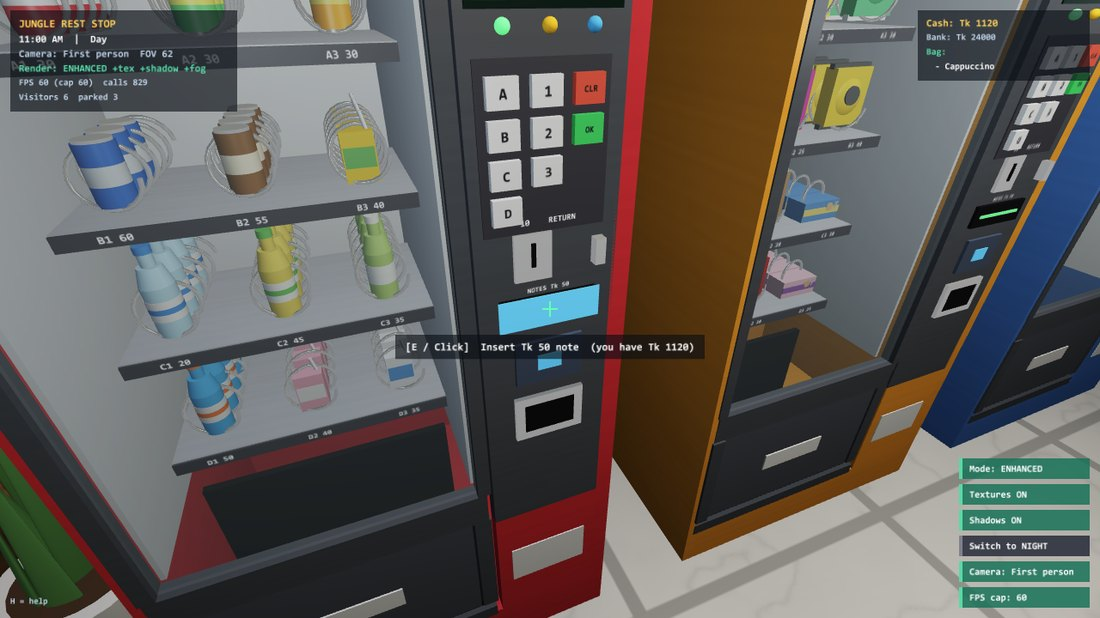
\includegraphics[width=\linewidth]{play_1_look}\caption{Looking at the note slot: ``Insert Tk 50 note''}\end{subfigure}
\begin{subfigure}{0.49\linewidth}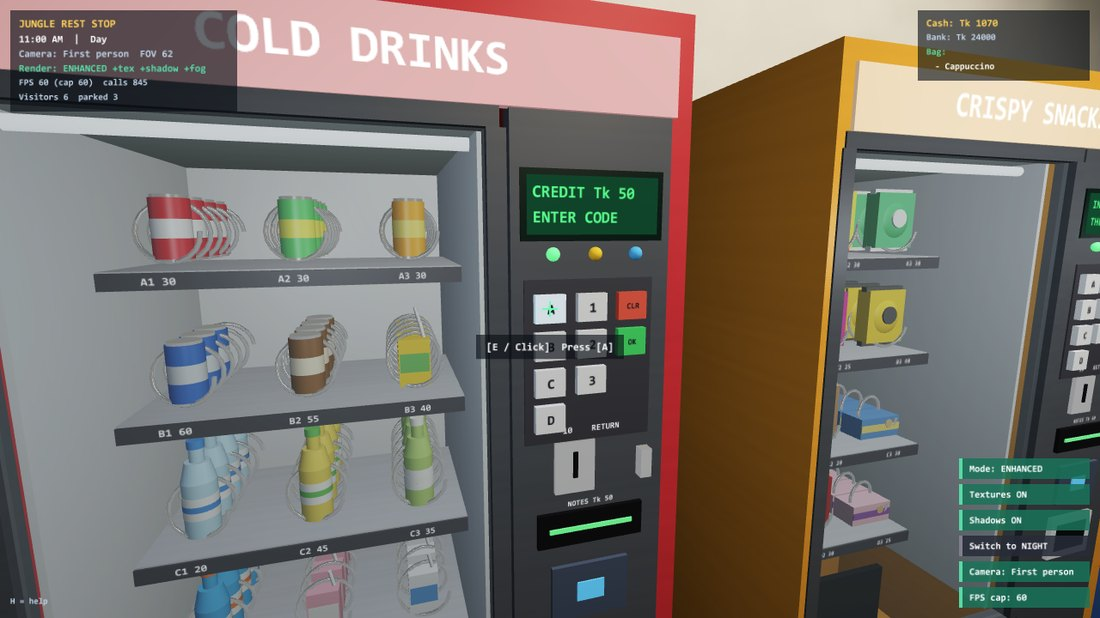
\includegraphics[width=\linewidth]{play_2_coin}\caption{Credit Tk 50 on the LCD; aiming at key A}\end{subfigure}
\begin{subfigure}{0.49\linewidth}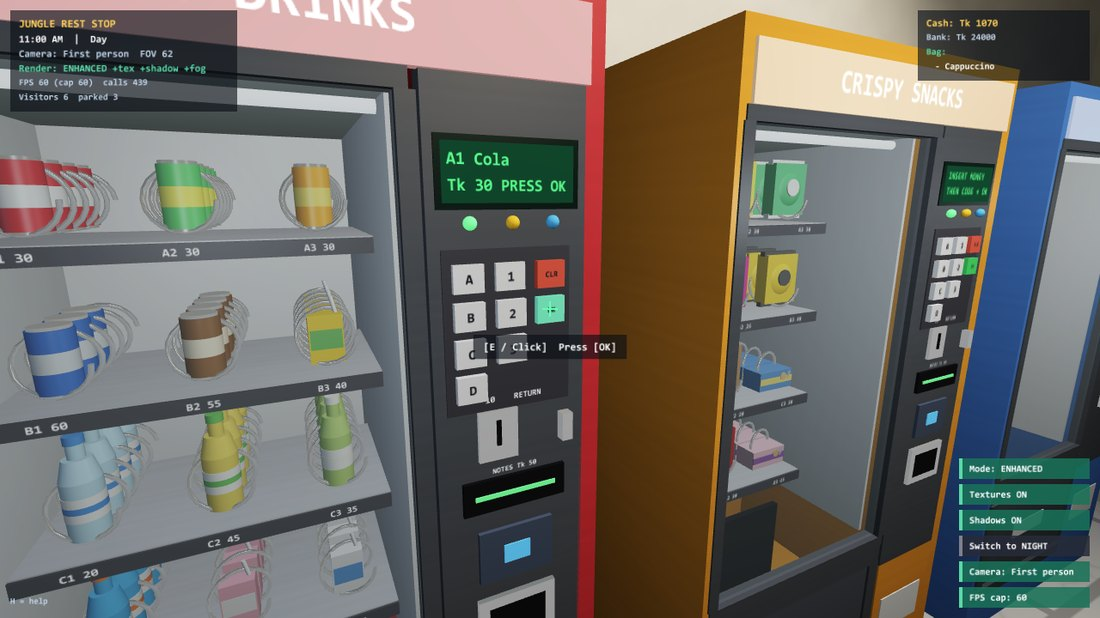
\includegraphics[width=\linewidth]{play_3_code}\caption{Code A1 (Cola, Tk 30) typed; aiming at OK}\end{subfigure}
\begin{subfigure}{0.49\linewidth}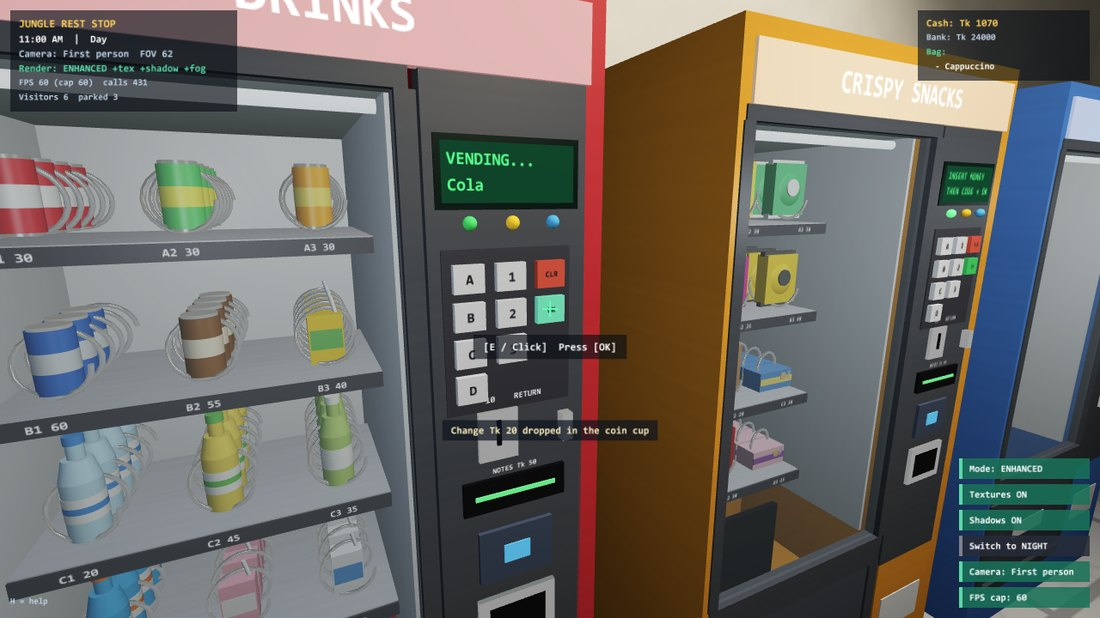
\includegraphics[width=\linewidth]{play_4_spiral}\caption{The spiral turns and pushes the can forward}\end{subfigure}
\begin{subfigure}{0.49\linewidth}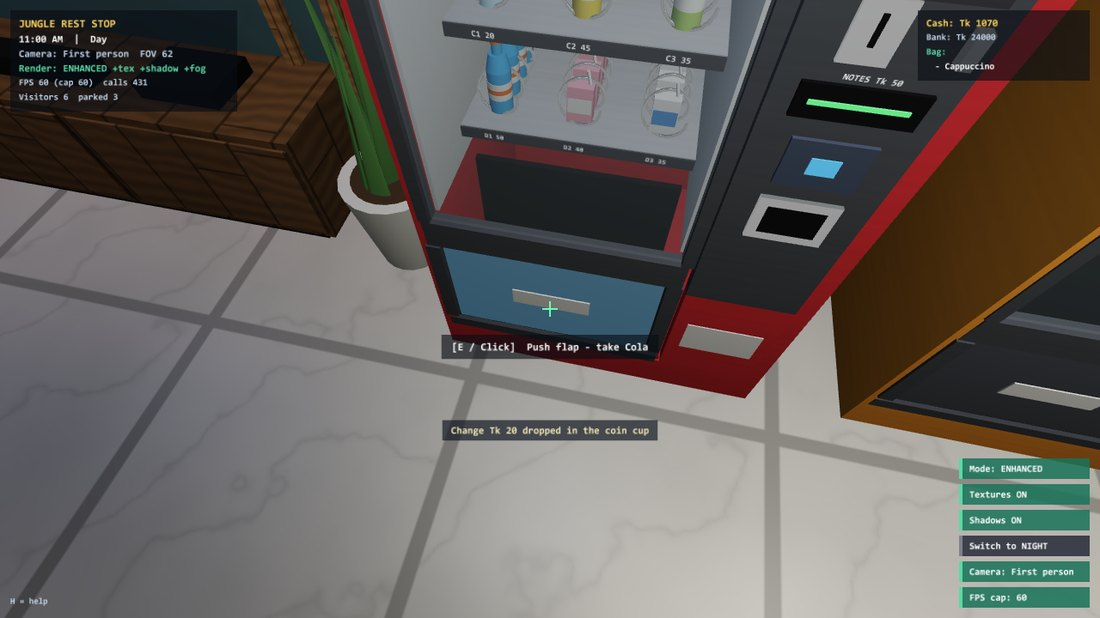
\includegraphics[width=\linewidth]{play_5_drop}\caption{The can lies in the tray: ``Push flap''}\end{subfigure}
\begin{subfigure}{0.49\linewidth}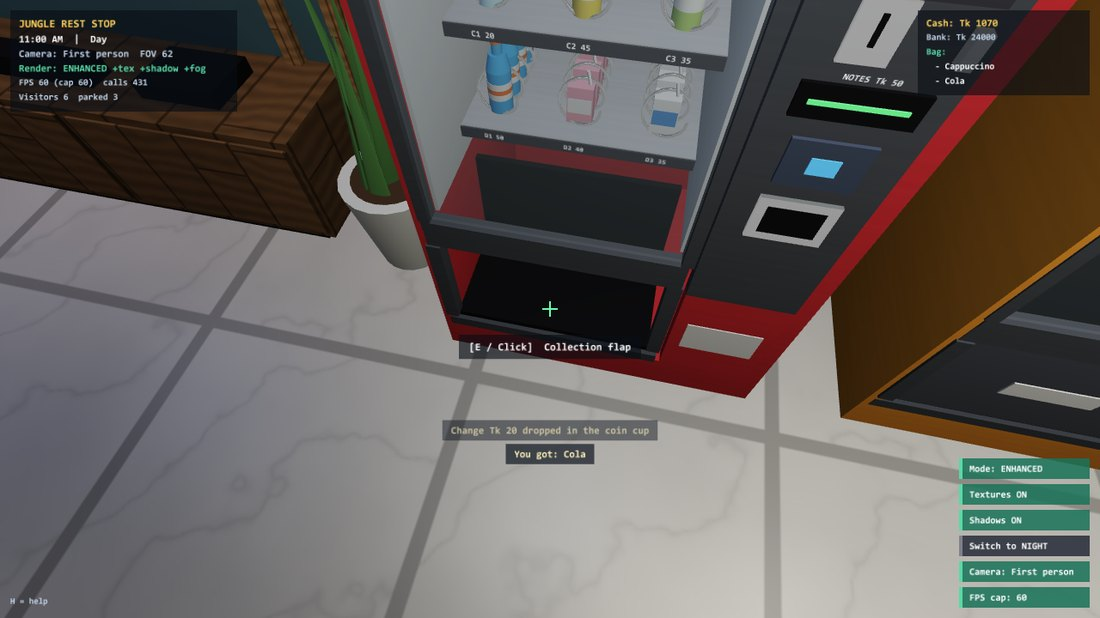
\includegraphics[width=\linewidth]{play_6_flap}\caption{The flap swings in; the can is in the bag, Tk 20 change in the cup}\end{subfigure}
\caption{The player buys a can of Cola.}\label{fig:playvend}
\end{figure}
\begin{figure}[H]
\centering
\begin{subfigure}{0.32\linewidth}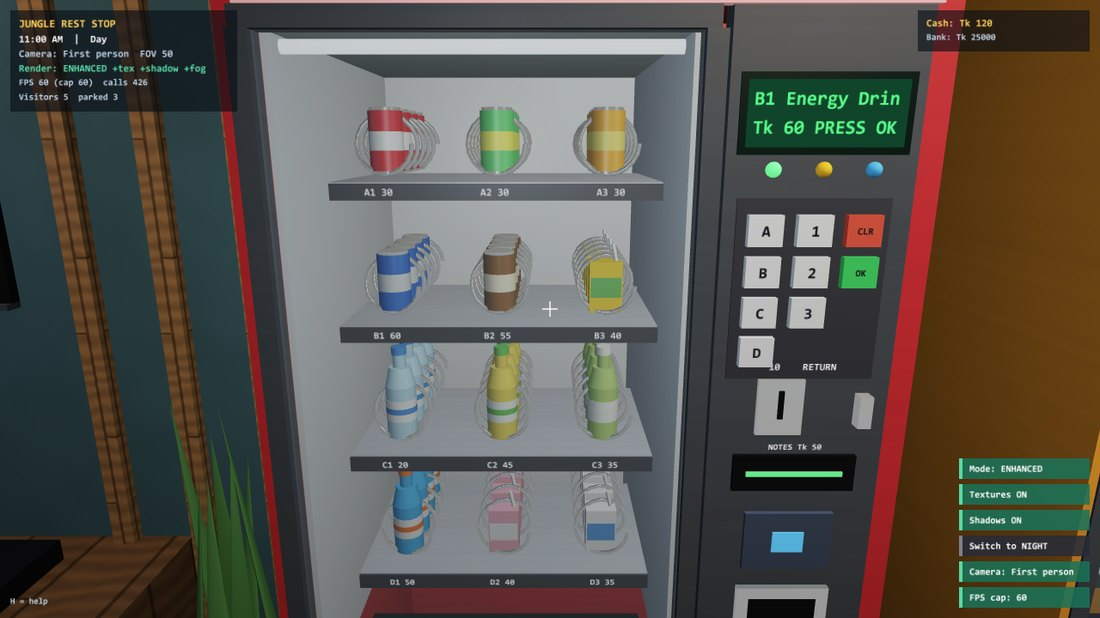
\includegraphics[width=\linewidth]{vending_code}\caption{Code typed, credit enough}\end{subfigure}
\begin{subfigure}{0.32\linewidth}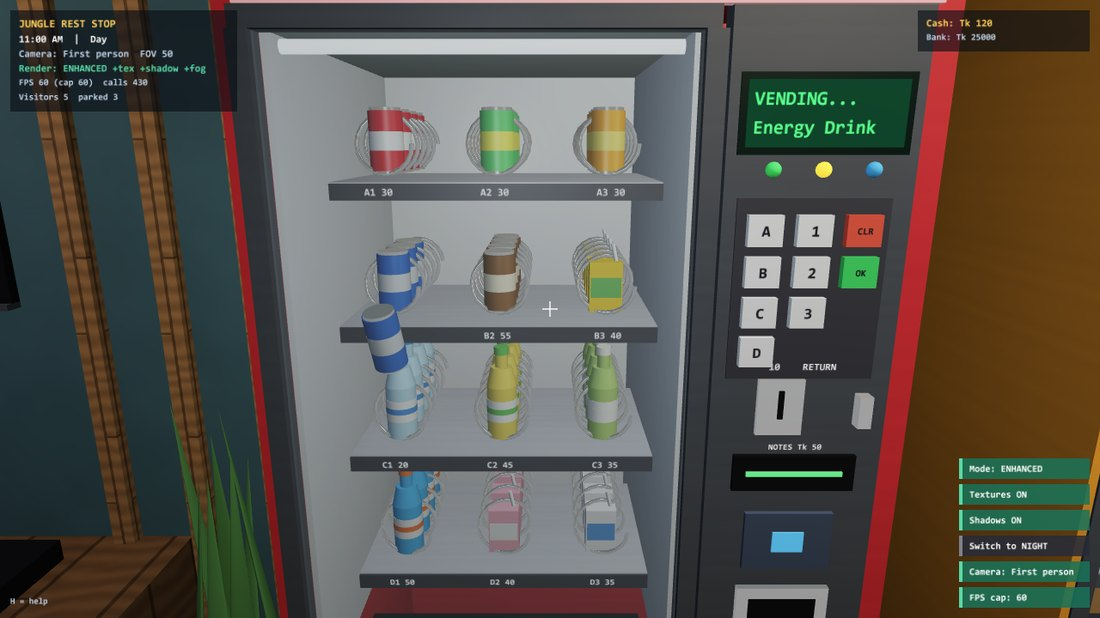
\includegraphics[width=\linewidth]{vending_dispense}\caption{The product falls}\end{subfigure}
\begin{subfigure}{0.32\linewidth}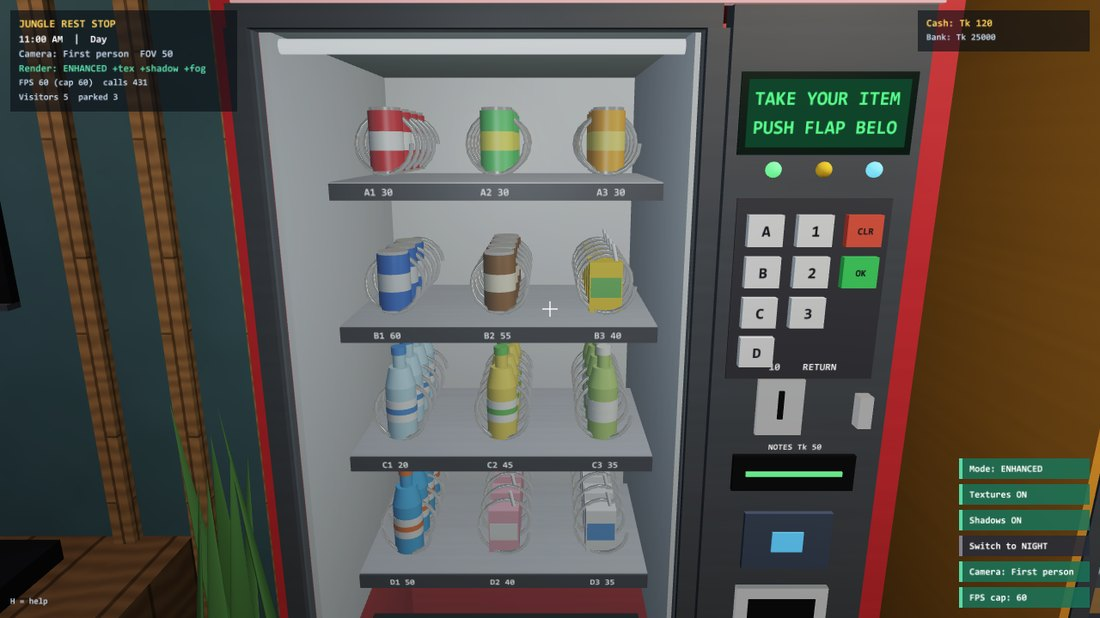
\includegraphics[width=\linewidth]{vending_ready}\caption{``Take your item''}\end{subfigure}
\caption{The same steps seen closer, with the downlight (spot light) above the machine.}\label{fig:vendbuy}
\end{figure}

\subsubsection{Using the ATM}
\begin{figure}[H]
\centering
\begin{tikzpicture}[state/.append style={minimum width=2.2cm,minimum height=0.75cm,font=\footnotesize},lb/.style={font=\scriptsize,fill=white,inner sep=1pt}]
\node[state] (w) at (0,0) {WELCOME};
\node[state] (c) at (2.8,0) {CARD IN};
\node[state] (p) at (5.6,0) {PIN + ENTER};
\node[state] (v) at (8.4,0) {VERIFY 1234};
\node[state] (m) at (11.2,0) {MENU};
\node[state=blue!8] (b) at (14.3,0) {BALANCE};
\node[state=red!10] (wr) at (7.0,1.5) {WRONG PIN};
\node[state] (a) at (11.2,-2.0) {AMOUNT};
\node[state] (pr) at (8.4,-2.0) {PROCESSING};
\node[state] (tc) at (5.6,-2.0) {TAKE CARD};
\node[state] (tm) at (2.8,-2.0) {TAKE CASH};
\node[state] (r) at (0,-2.0) {RECEIPT};
\node[state] (t) at (0,-3.6) {THANK YOU};
\draw[arr] (w)--(c); \draw[arr] (c)--(p); \draw[arr] (p)--(v); \draw[arr] (v)--(m);
\draw[arr] (v.north) |- (wr.east);
\draw[arr] (wr.west) -| (p.north);
\draw[arr] (m)--node[lb,right]{Withdraw}(a);
\draw[arr] (m)--(b);
\draw[arr] (b.north) -- ++(0,0.45) -| node[lb,above,pos=0.25]{Back} (m.north);
\draw[arr] (b.south) |- node[lb,pos=0.25,right]{Exit} ([yshift=-0.75cm]tc.south) -- (tc.south);
\draw[arr] (a)--(pr); \draw[arr] (pr)--(tc); \draw[arr] (tc)--(tm); \draw[arr] (tm)--(r); \draw[arr] (r)--(t);
\draw[arr] (t.west) -- ++(-0.5,0) |- (w.west);
\end{tikzpicture}
\caption{ATM state machine. CANCEL at any step leads to TAKE CARD; the card is always returned before the cash.}\label{fig:atmsm}
\end{figure}
The eight steps are listed in a HUD panel and the current step is highlighted. Inside the machine the card slides in
and out, the PIN appears as stars, the notes slide out of the dispenser and the receipt curls out of the printer.
\begin{figure}[H]
\centering
\begin{subfigure}{0.32\linewidth}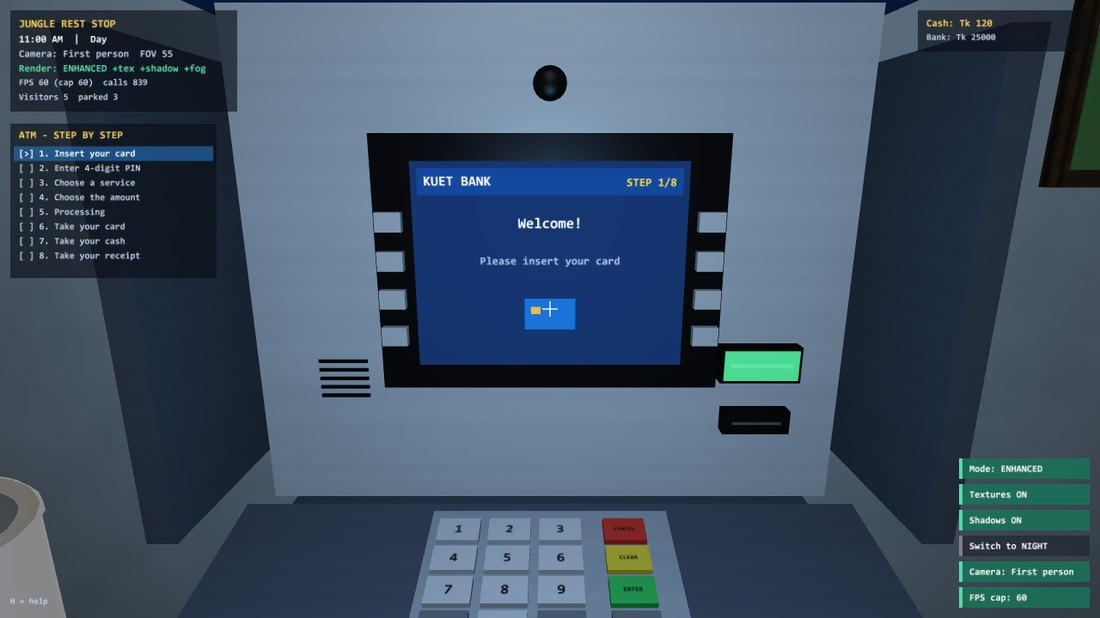
\includegraphics[width=\linewidth]{atm_1_welcome}\caption{1. Insert card}\end{subfigure}
\begin{subfigure}{0.32\linewidth}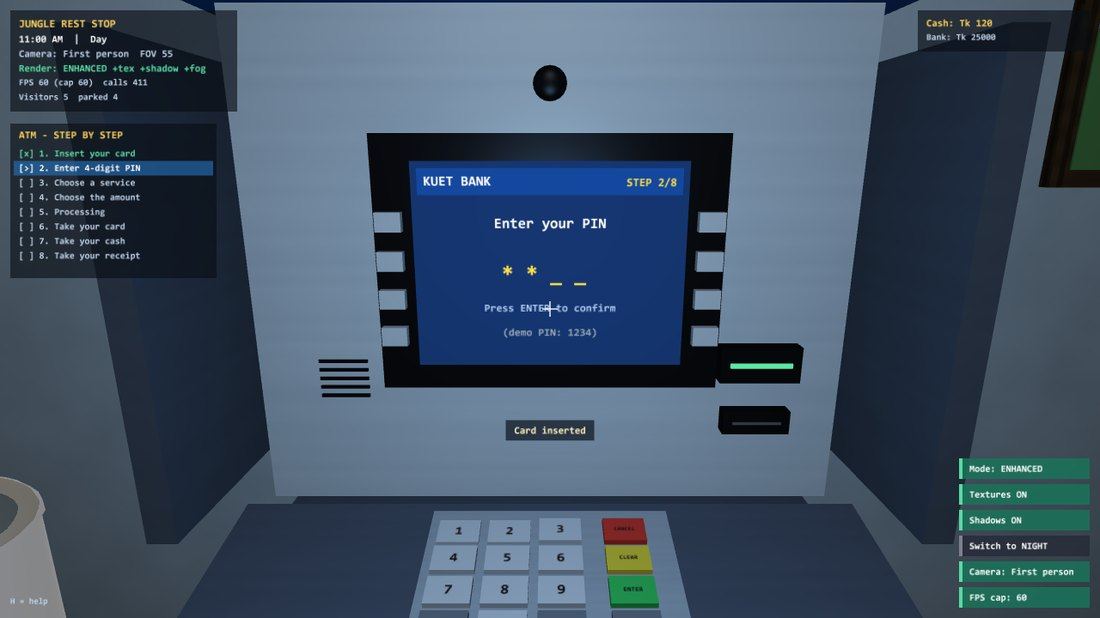
\includegraphics[width=\linewidth]{atm_2_pin}\caption{2. Enter PIN}\end{subfigure}
\begin{subfigure}{0.32\linewidth}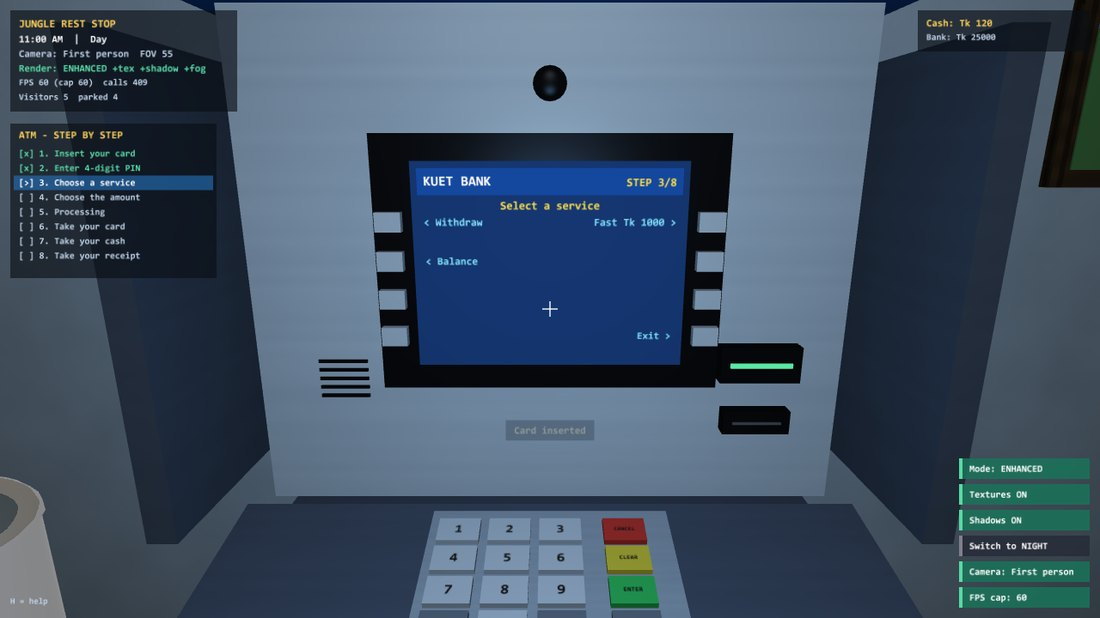
\includegraphics[width=\linewidth]{atm_3_menu}\caption{3. Choose a service}\end{subfigure}
\begin{subfigure}{0.32\linewidth}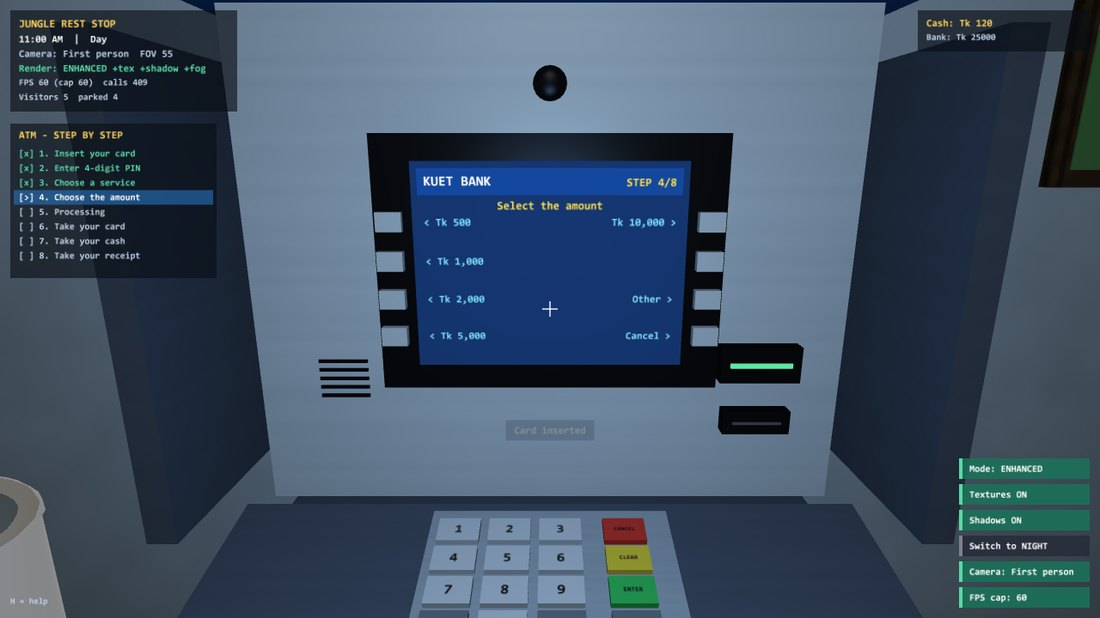
\includegraphics[width=\linewidth]{atm_4_amount}\caption{4. Choose amount}\end{subfigure}
\begin{subfigure}{0.32\linewidth}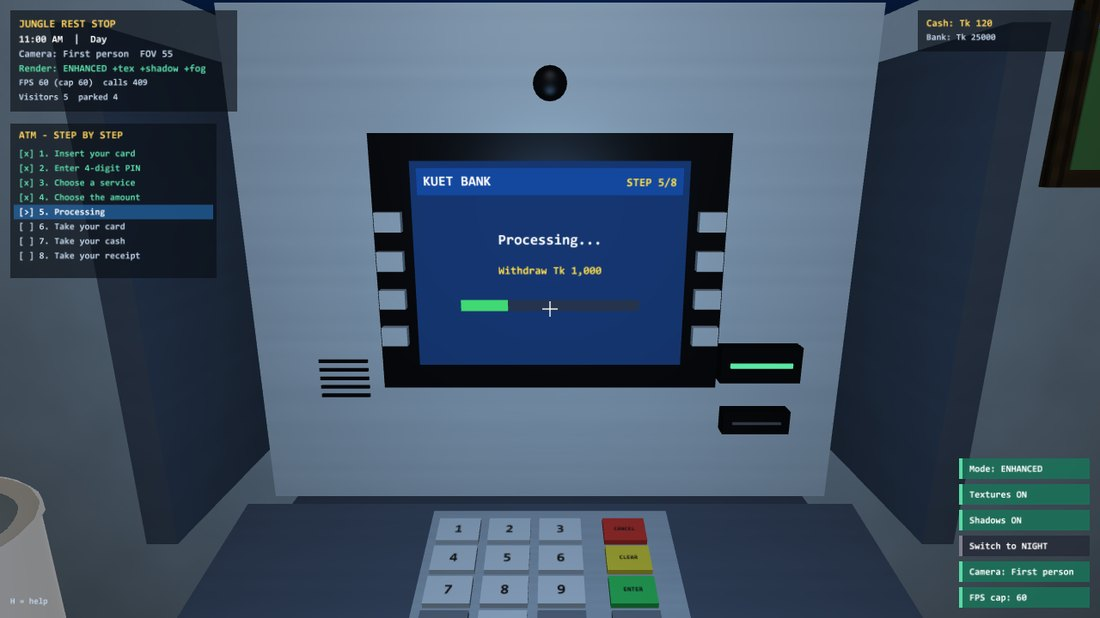
\includegraphics[width=\linewidth]{atm_5_processing}\caption{5. Processing}\end{subfigure}
\begin{subfigure}{0.32\linewidth}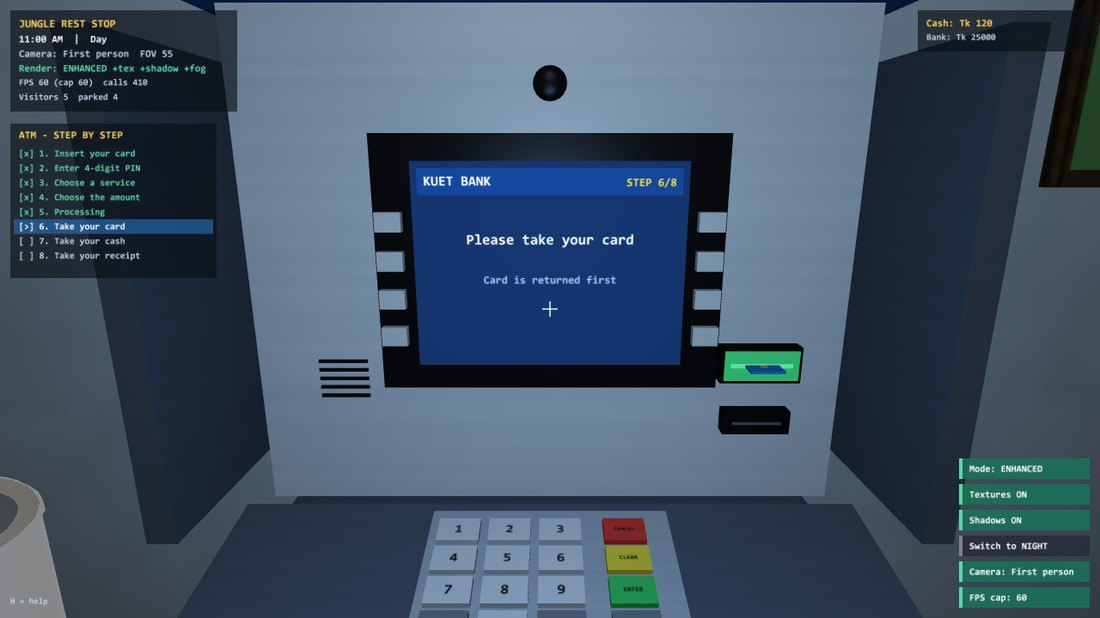
\includegraphics[width=\linewidth]{atm_6_takecard}\caption{6. Take card}\end{subfigure}
\begin{subfigure}{0.32\linewidth}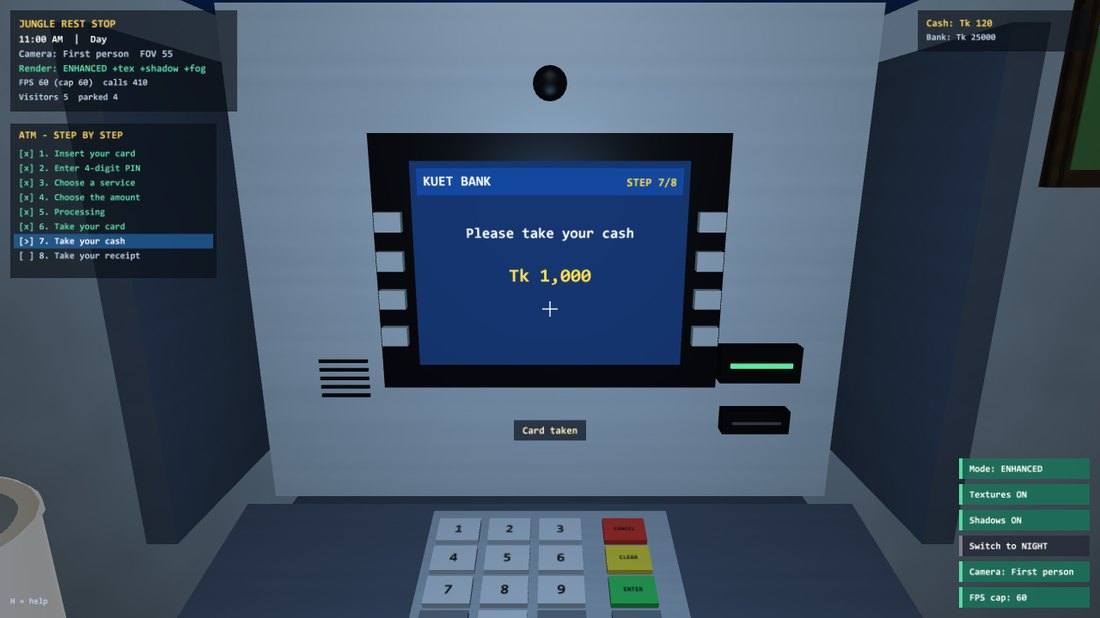
\includegraphics[width=\linewidth]{atm_7_takecash}\caption{7. Take cash}\end{subfigure}
\begin{subfigure}{0.32\linewidth}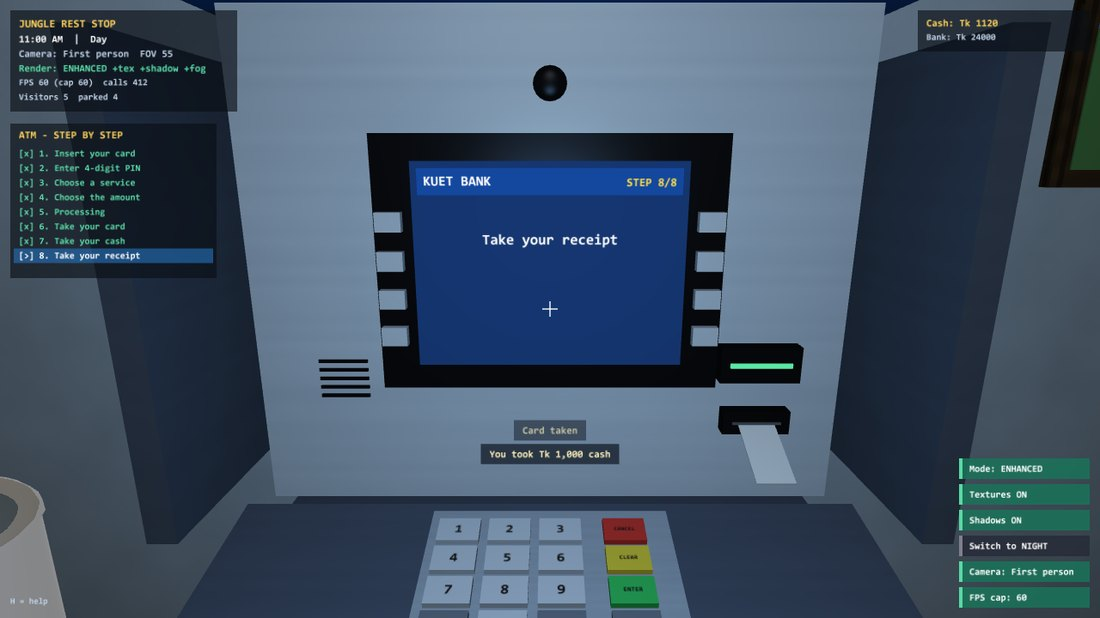
\includegraphics[width=\linewidth]{atm_8_receipt}\caption{8. Take receipt}\end{subfigure}
\begin{subfigure}{0.32\linewidth}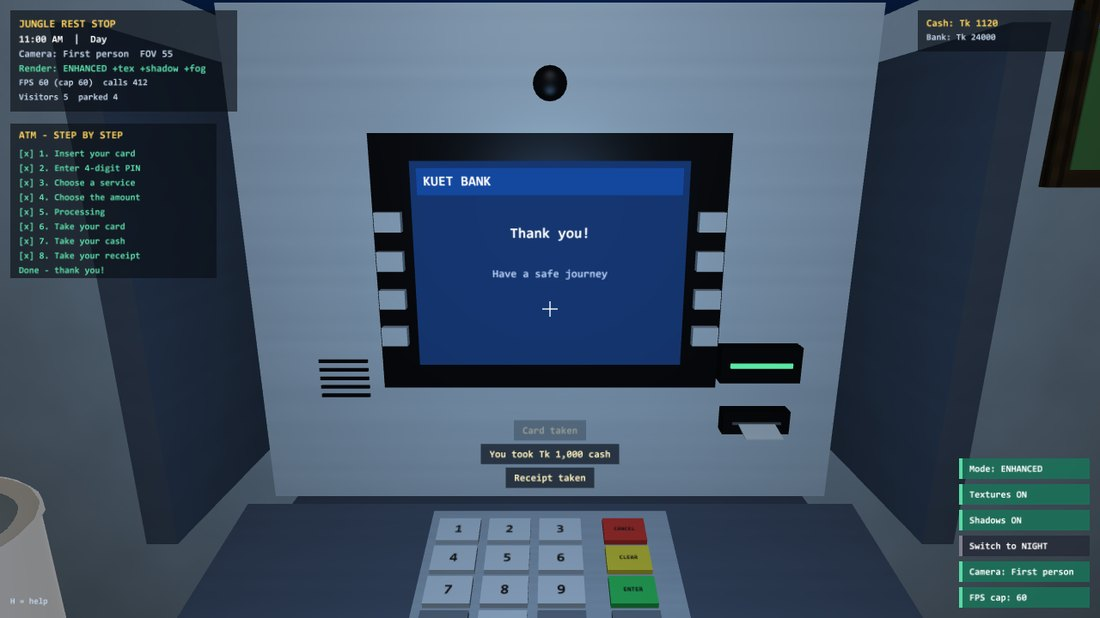
\includegraphics[width=\linewidth]{atm_9_thanks}\caption{Done}\end{subfigure}
\caption{A withdrawal of Tk 1,000 with the step list on the left.}
\end{figure}

\subsubsection{Coffee machine, television, light switch and aquarium}
\begin{figure}[H]
\centering
\begin{subfigure}{0.49\linewidth}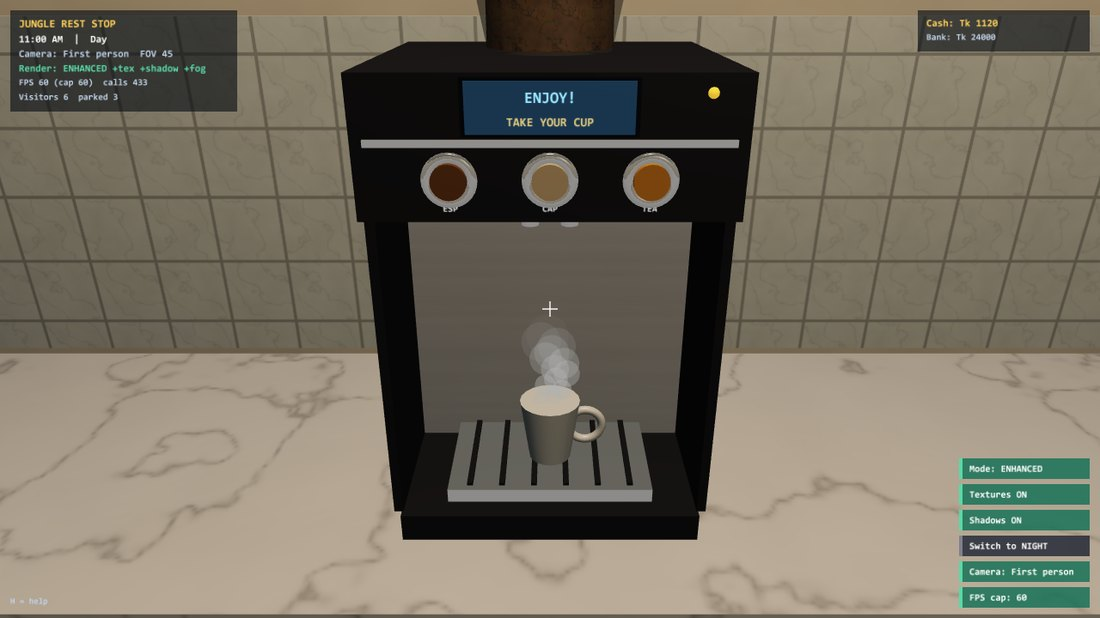
\includegraphics[width=\linewidth]{coffee_brewing}\caption{Brewing a cappuccino (stream, rising coffee, steam)}\end{subfigure}
\begin{subfigure}{0.49\linewidth}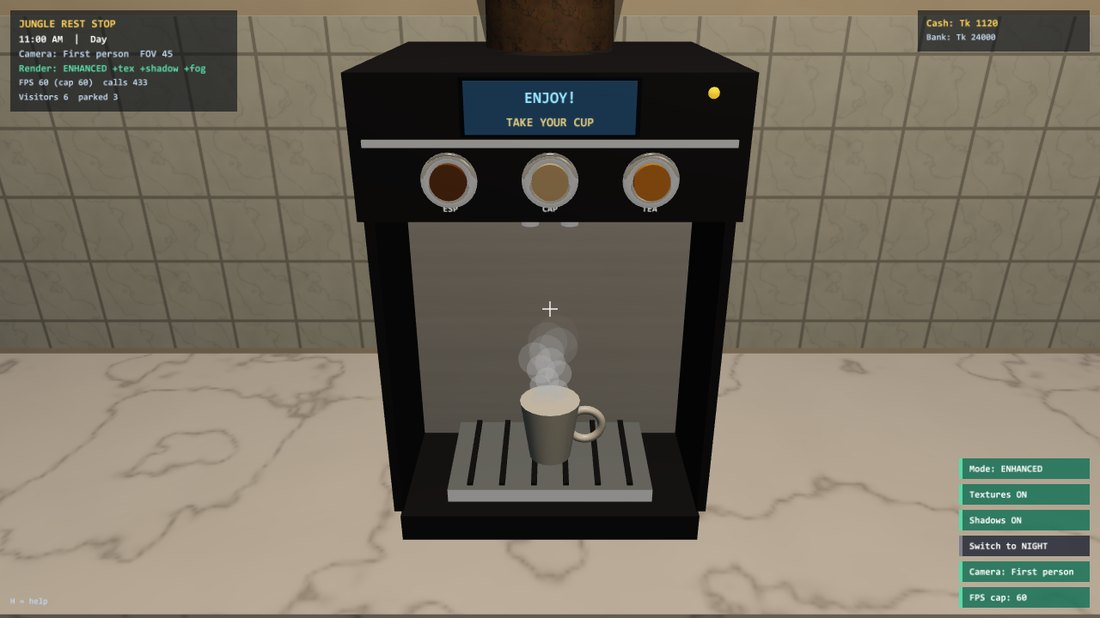
\includegraphics[width=\linewidth]{coffee_ready}\caption{Ready: take the cup}\end{subfigure}
\begin{subfigure}{0.49\linewidth}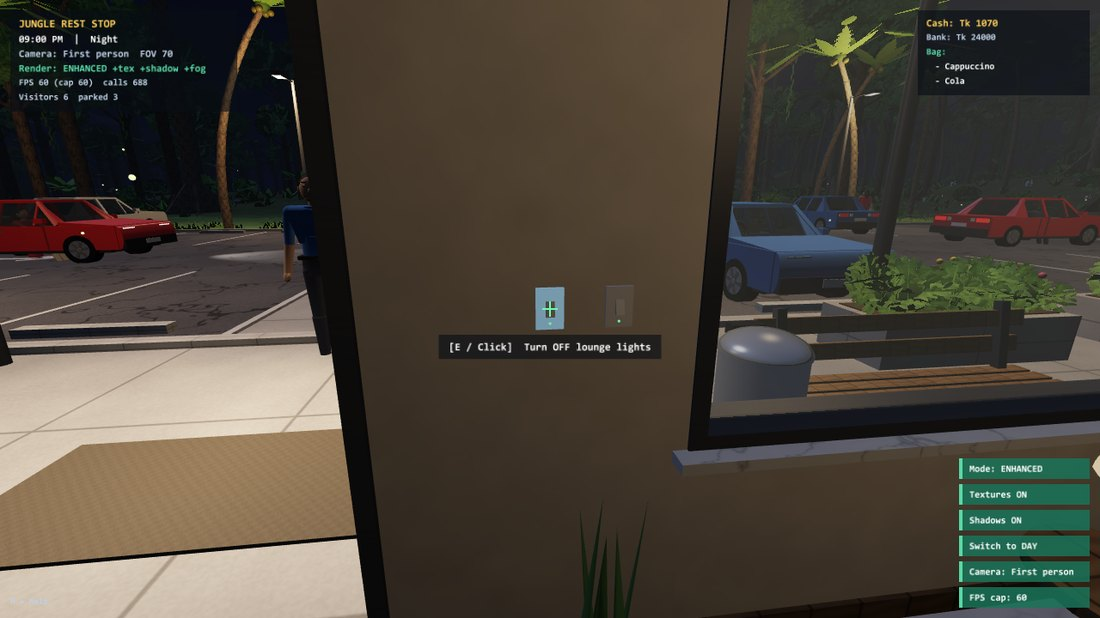
\includegraphics[width=\linewidth]{play_switch_on}\caption{Night: looking at the lounge light switch}\end{subfigure}
\begin{subfigure}{0.49\linewidth}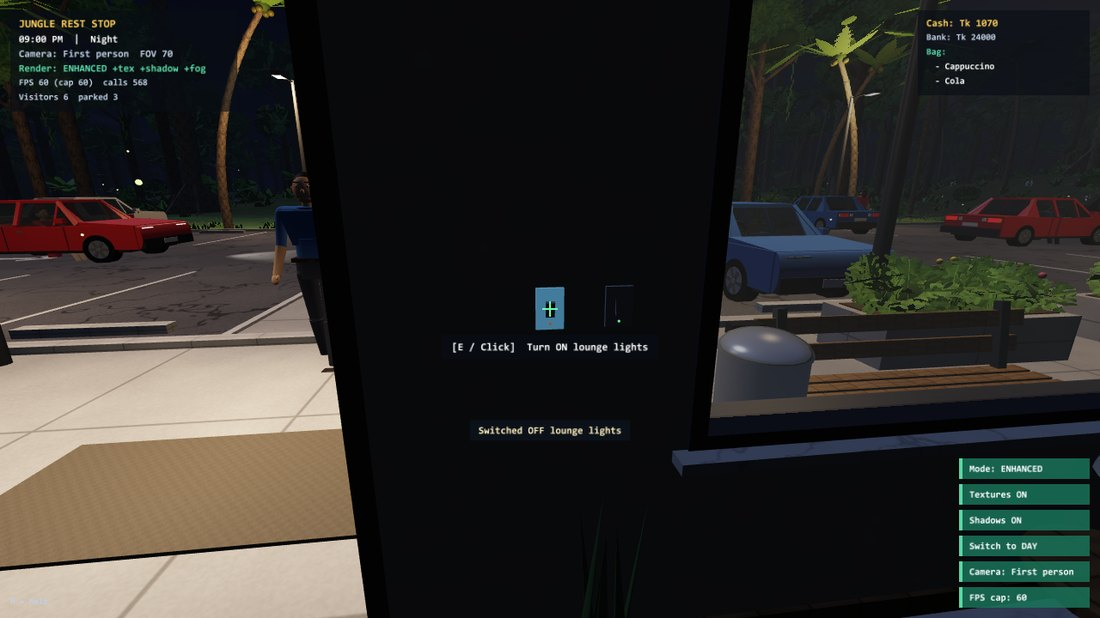
\includegraphics[width=\linewidth]{play_switch_off}\caption{After pressing E: the lounge lights are off}\end{subfigure}
\begin{subfigure}{0.49\linewidth}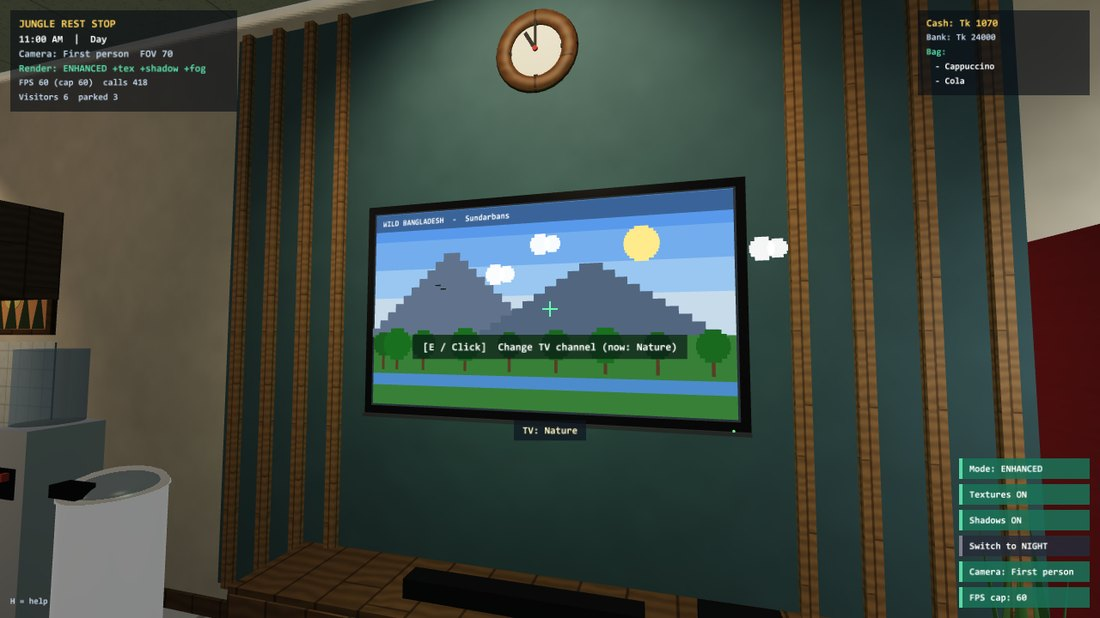
\includegraphics[width=\linewidth]{play_tv}\caption{Changing the TV channel}\end{subfigure}
\begin{subfigure}{0.49\linewidth}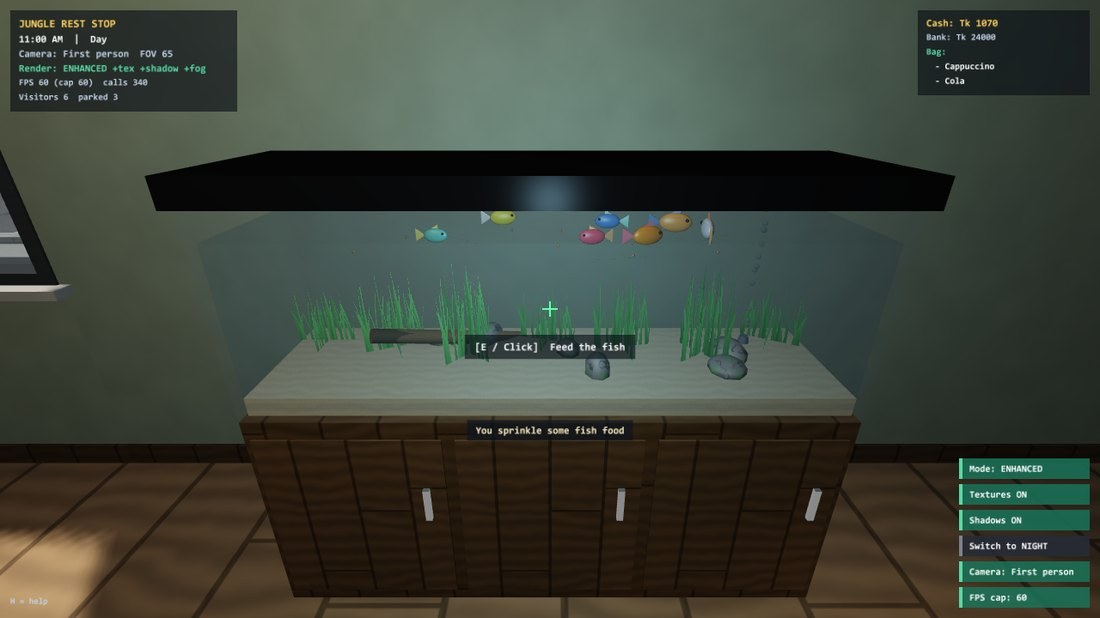
\includegraphics[width=\linewidth]{play_fish}\caption{Feeding the fish: they swim up to the food}\end{subfigure}
\caption{Reactions of the coffee machine, the light switch, the TV and the aquarium.}
\end{figure}
\begin{figure}[H]
\centering
\begin{subfigure}{0.24\linewidth}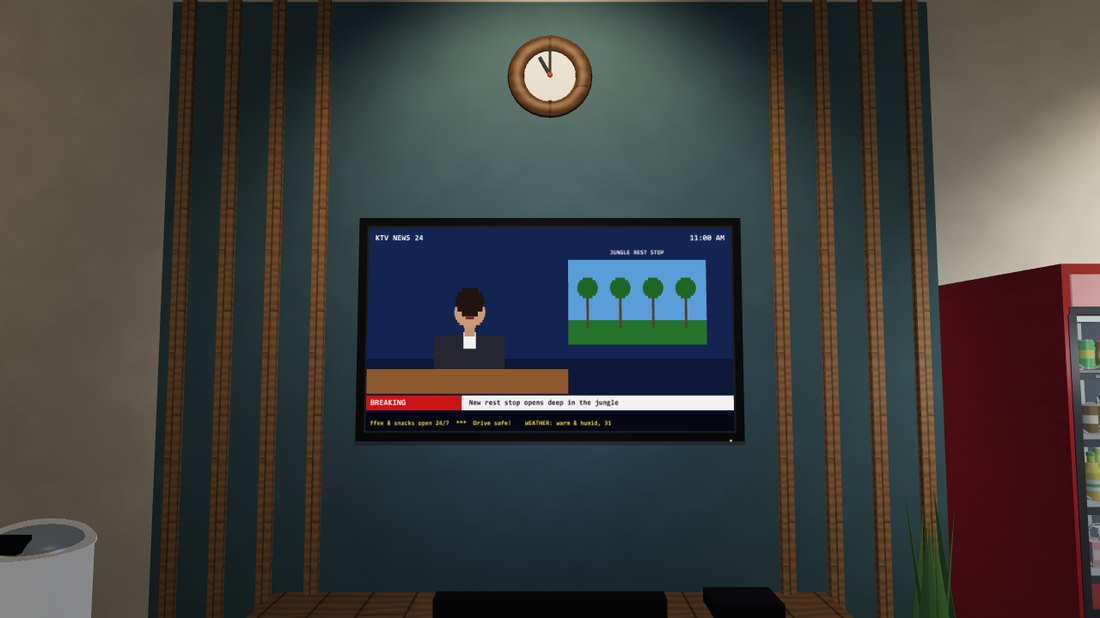
\includegraphics[width=\linewidth]{tv_ch1}\caption{News + ticker}\end{subfigure}
\begin{subfigure}{0.24\linewidth}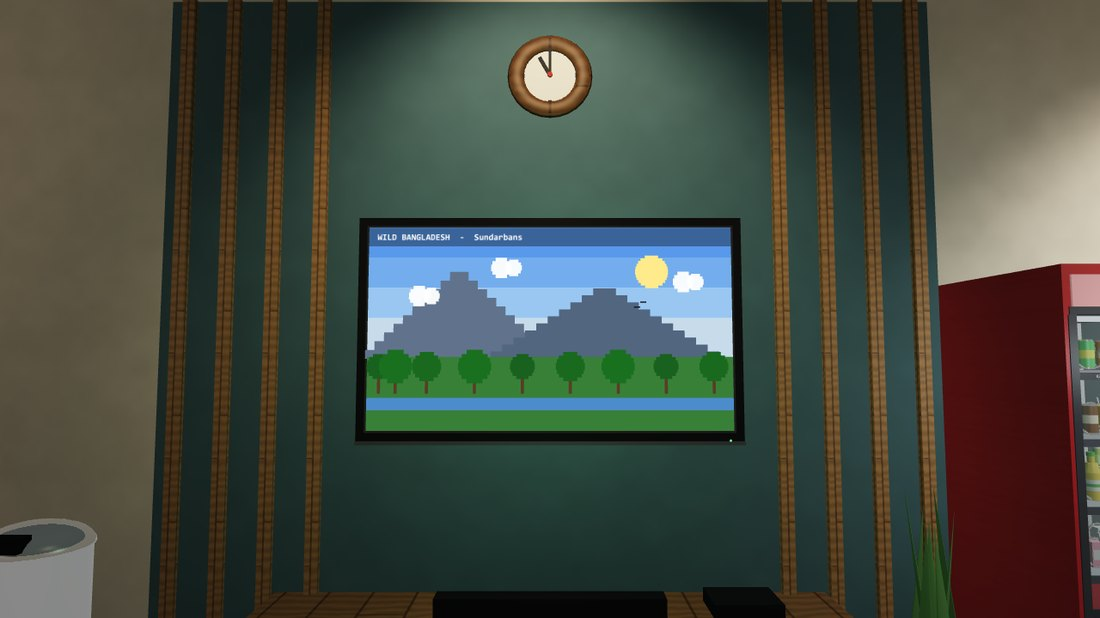
\includegraphics[width=\linewidth]{tv_ch2}\caption{Nature}\end{subfigure}
\begin{subfigure}{0.24\linewidth}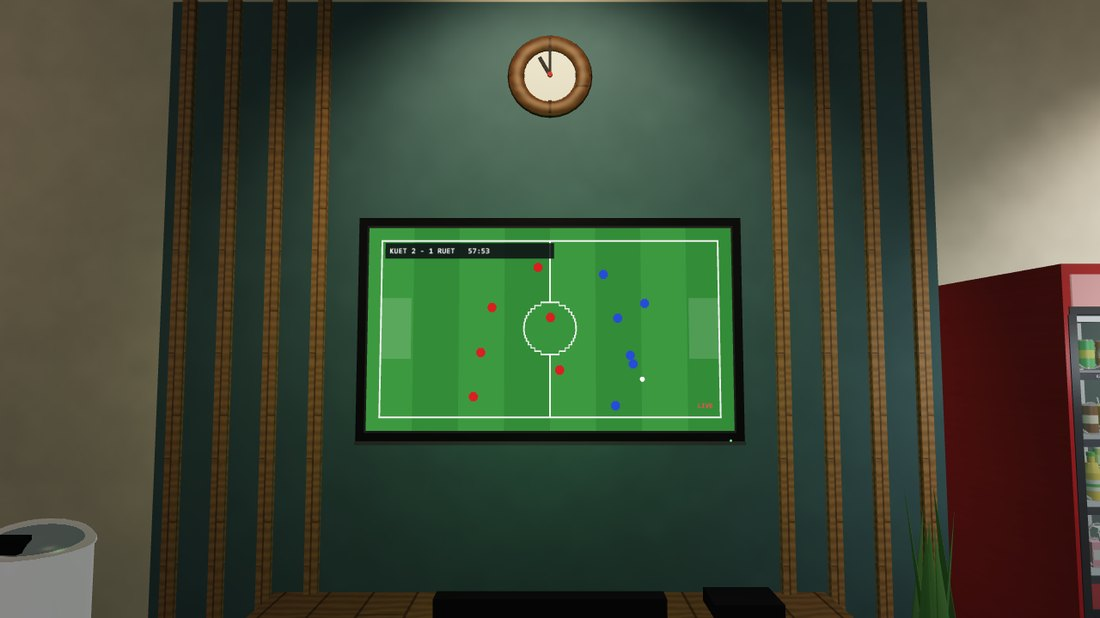
\includegraphics[width=\linewidth]{tv_ch3}\caption{Live football}\end{subfigure}
\begin{subfigure}{0.24\linewidth}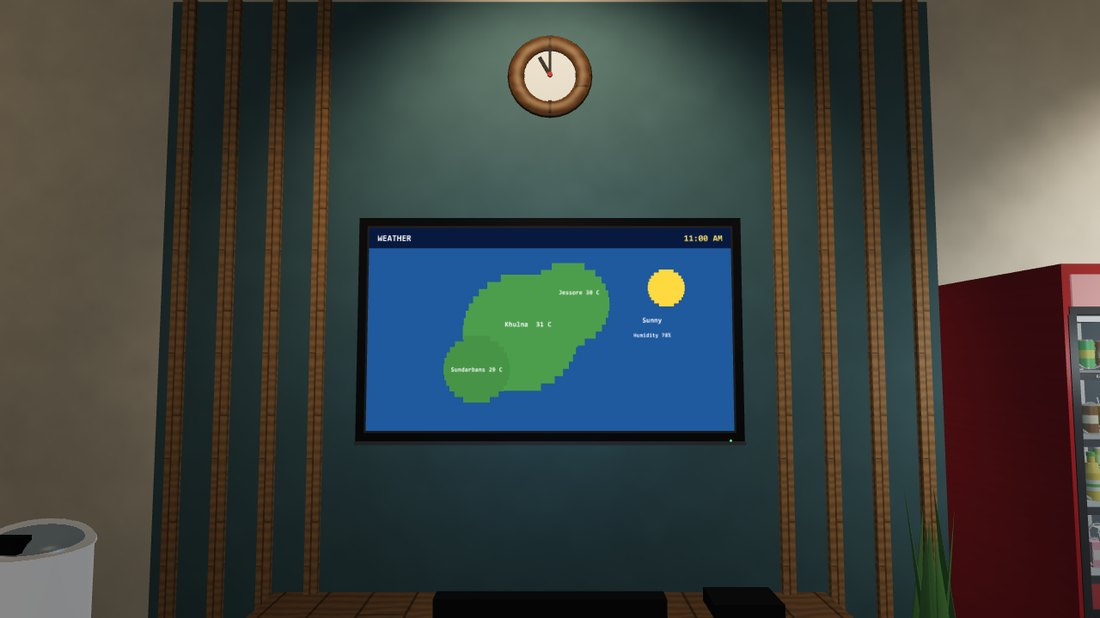
\includegraphics[width=\linewidth]{tv_ch4}\caption{Weather (game time)}\end{subfigure}
\caption{The four animated TV channels.}
\end{figure}
